%%%%%%%%%%%%%%%%%%%%%%%%%%%%%%%% 
\section{Beam Line Measurements} 
\label{sec:detectors-nd-ref-blm}

This chapter outlines the DUNE strategy for measurements of secondary
beam particles in the region behind the beam absorber. 
Those measurements are designed to provide constraints 
on the neutrino flux at the near and far
detectors, and data on the pulse-to-pulse variation
of the beam for beam diagnostic purposes. A description of equipment
for monitoring the proton beam's interaction with the proton target
can be found in Volume 2: The Beamline at the Near Site. 

The measurements and apparatus described in this chapter fall into
the category of equipment designed specifically for DUNE to
detect muons exiting the decay tunnel. 

\subsection{Design Considerations}
\label{subsec:detectors-nd-blm-design}

The requirements for the beamline measurements, 
as discussed in the NDC requirements documentation~\cite{nd_requirements_doc}, \fixme{old LBNE reference}
are intimately related to how well the neutrino flux must be known. 
Given that DUNE does not have the luxury to construct identical 
Near and Far Detectors, a near-far comparison is more complicated than it was in
the MINOS experiment~\cite{gnumi-validation}, for example.   
While external hadron-production measurements can place strong 
constraints on the pion and kaon production in the target, they do not 
provide any confirmation of the simulation of other key features, such 
as the horn focusing, secondary interactions, and the 
pion scattering and absorption in the air-filled decay volume. 

In addition to the external measurements, covered in Section~\ref{sec:detectors-nd-external-hadron}, 
that confirm the simulation of the thick target, horn material, decay tunnel and
absorber, it is desirable to constrain the flux by making independent
measurements at the 4--5\% level of the muons that penetrate the absorber. It would not be practical to do this for all penetrating muons, but sufficient measurements at a few positions can be done in a  cost-effective way. 
%
%\subsubsection{Muon Measurements}
%\label{subsubsec:detectors-nd-blm-muon-meas}

The primary physics goal of DUNE is to measure the transmutation
of $\nu_\mu$s to $\nu_e$s over the 1300km between Fermilab
and the far detector site.
Therefore it is essential for DUNE to cross-check the estimate of 
background $\nu_e$s present in the beam by using several
methods to measure their rates at the Fermilab site. 
There are two dominant sources of $\nu_e$s present in the
neutrino beam, muon decays and kaon decays. 
The muon systems are designed to directly measure the 
muons that penetrate absorber with an energy 
threshold as low as possible, i.e. directly measure those muons 
whose decays are a major source of background $\nu_e$s. 
A measurement of the spectrum of those muons will translate
 directly into constraints on the spectrum of background $\nu_e$s.
That constraint has the enormous advantage of being independent of poorly understood 
neutrino-nucleus cross sections.

Because muons and neutrinos come from the same parent pion and kaon
decays, a measurement of the absolute muon flux in conjunction with the energy spectrum
seen in the muon monitors can constrain the absolute neutrino flux.  
The goal for the DUNE muon monitors is to determine the absolute muon flux
to an accuracy of 5\% above a muon energy of 6~GeV (which corresponds to
a neutrino energy of 1.6~GeV) in the central part of the absorber.

It is essential to monitor the stability of the beam direction over
time. For example, above 6~GeV, the ratio of the Far Detector flux over 
the Near Detector flux changes by 2\%.  
To keep the change in the neutrino beam less than 1\% in all energy bins,
the beam direction must be known to a precision of approximately 0.2~mrad. 
Because the muon monitors will be located approximately 275~m
from the beam target, this requires a measurement of the muons to an
accuracy of approximately 5~cm.

%
%
%%%%%%%%%%%%%%%%%%%%%%%%%%%%%%%%%%%%%%%%%%%%%%%%%%%%%%%
\subsection{Muon-Measurement Facilities}
\label{subsec:detectors-nd-blm-muon-measurement-facilities}

The muon measurements are carried out in the region immediately
following the hadron absorber at the end of the decay tunnel, below
the Absorber Service Building (LBNF 30).  A view
of the absorber area and the muon alcove is shown in Figure~\ref{fig:AbsorberElevationView}. 
The axis of the decay pipe cuts across the muon alcove at an angle, and the size of the alcove
is largely determined by the requirement that it contain the
shadow of the four-meter-diameter decay pipe, projected through the
alcove, as shown in the elevation view of Figure~\ref{fig:AbsorberElevationView}. 

Figure~\ref{fig:AbsorberElevationView} shows the downstream side of the
absorber and a conceptual layout of the muon systems described in various sections of this
chapter.  
The absorber itself is encased in concrete. The first set of
muon-measurement devices, from left to right, is a
 variable-pressure gas Cherenkov counters, which 
mounted on a movable stand in order to scan across the rear surface of the absorber.
 Following that is an
array of diamond ionization detectors and finally a set of stopped-muon 
counters which are interspersed between walls of
steel ``blue blocks''.   The blue blocks are there to provide several
depths at which to monitor the stopped muons as they range out in the
material. A second array of ionization devices will also be placed farther downstream within the blue blocks.

\begin{cdrfigure}[Absorber conceptual design, elevation view]{AbsorberElevationView}
{Absorber conceptual design. The figure shows the elevation view of the 
absorber at the end of the decay tunnel. The beam axis is shown by
the blue line. The absorber is constructed of several different 
materials as shown: aluminum core in blue and grey, concrete 
(grey and tan), and steel (in brown and green).}
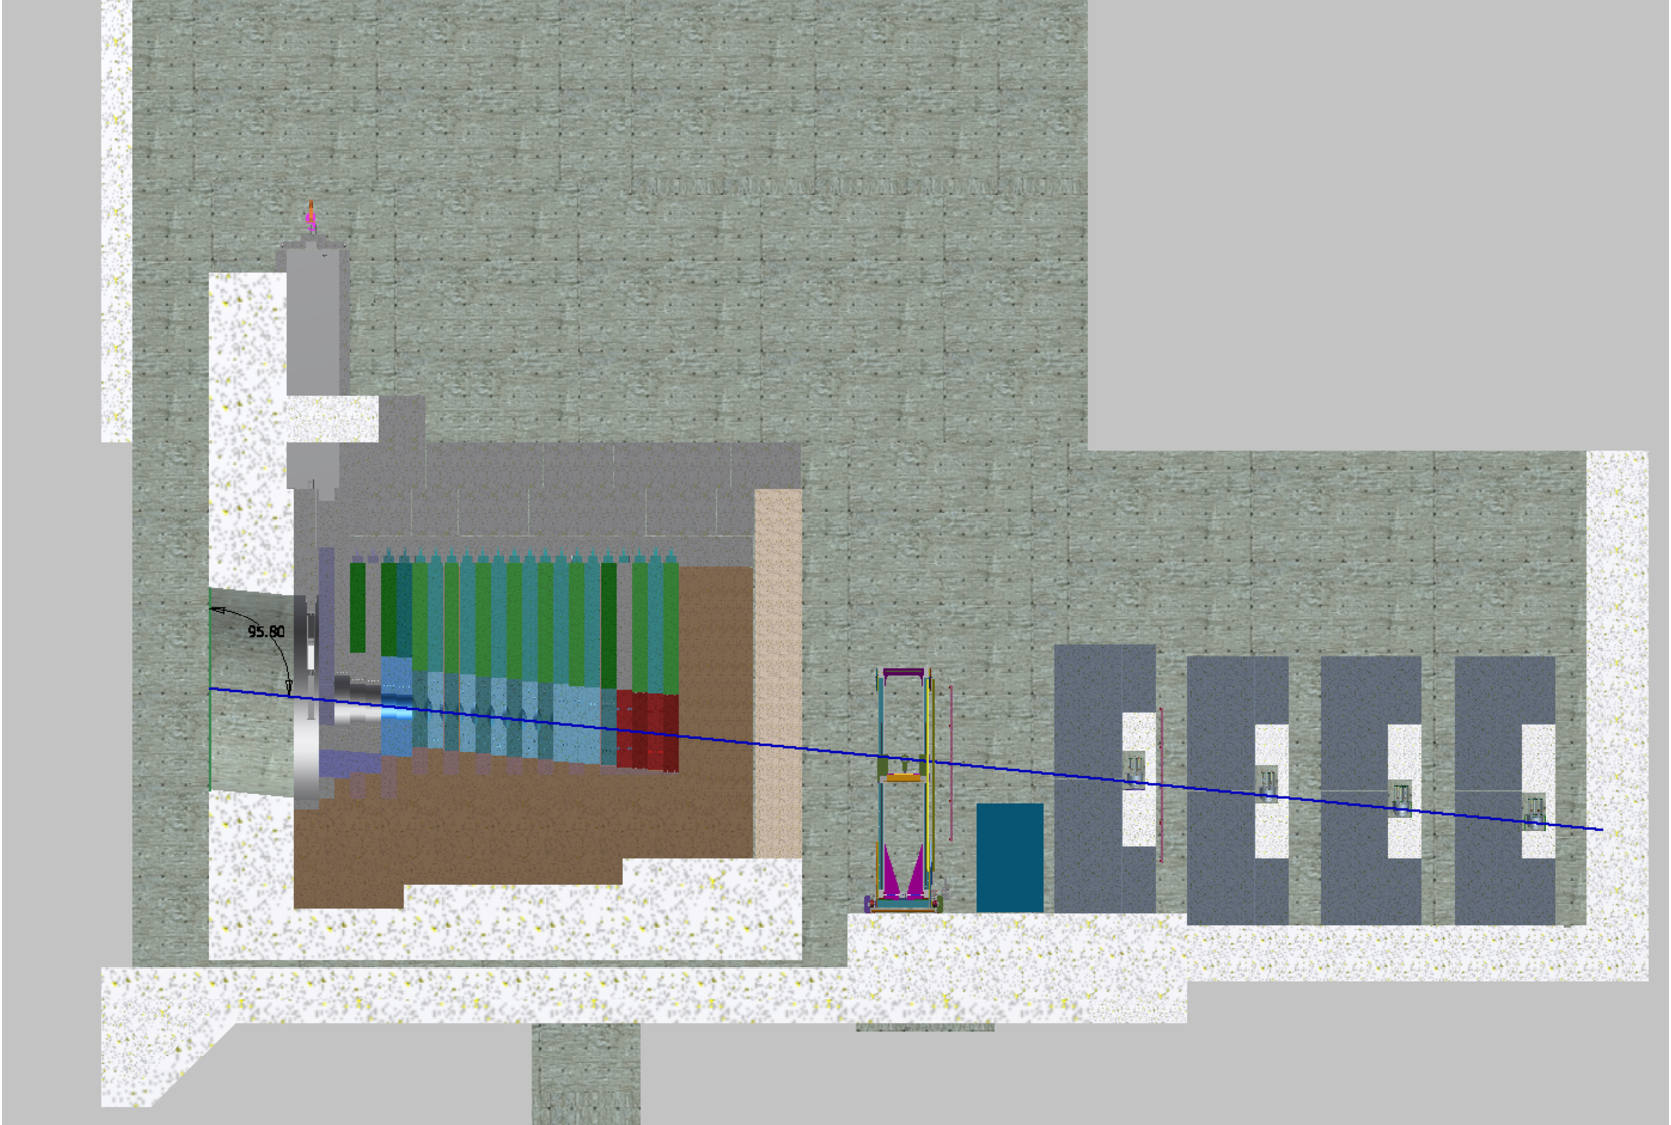
\includegraphics[width=4in,angle=0]{AbsorberElevationView}
\end{cdrfigure}

Figure~\ref{fig:AbsorberThickness} shows the energy lost by a
horizontal muon as it traverses the absorber, as a function of the
distance from the beam axis along a 45$^\circ$ line perpendicular to the beam axis. 
In the central region, roughly to a distance of  105~cm, the muons lose between 5.0 to 6.4~GeV, so that the
lowest-energy muons leaving the absorber at that point correspond to
neutrino energies of $\sim$ 1.5 to 2.0~GeV. At a radius of roughly 105~cm, the
full thickness of steel causes the muons 10~GeV or more,
corresponding to neutrino energies of $\sim$ 2.6~GeV. From the
perspective of the muon systems it will be desirable to lower these
thresholds if possible. 

\begin{cdrfigure}[Energy loss in absorber]{AbsorberThickness}{The energy loss a muon, parallel to the beam axis, experiences as it traverses the material in the absorber. The muon's energy loss is plotted versus the distance from the beam axis, along a 45 $^\circ$ line perpendicular to the beam axis. Muons suffer between 4.7 and 9.3~GeV of energy loss depending upon where they cross the absorber.}
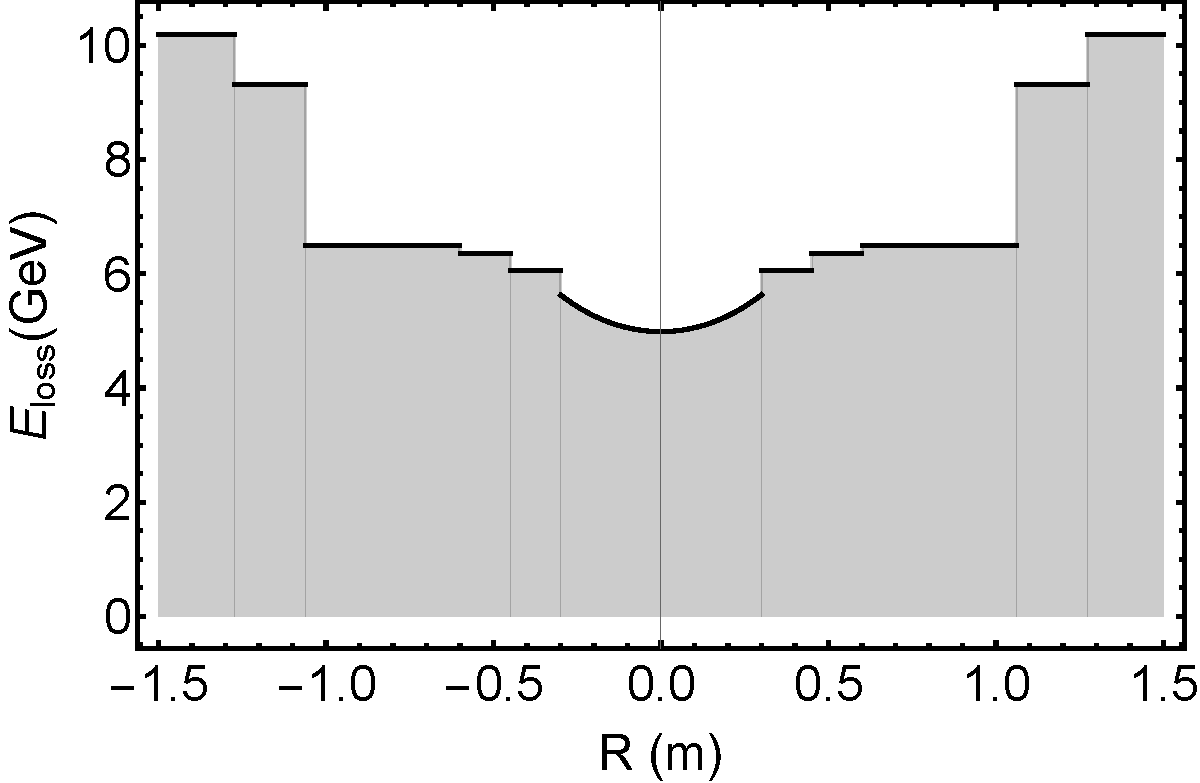
\includegraphics[width=4in,angle=0]{AbsorberThickness}
\end{cdrfigure}

%
%
%%%%%%%%%%%%%%%%%%%%%%%%%%%%%%%%%%%%%%%%%%%%%%%%%%%%%%%
\subsection{Muon Cherenkov Detector Reference Design} % (WBS 130.03.03.04)}
\label{sec:nd-blm-muon-cherenkov}

A Cherenkov variable-pressure, gas Cherenkov counter, operated in differential mode
will be deployed downstream of the absorber.  The counter will be mounted on a movable 
stand that will allow the system to scan in a plane transverse to the beam axis. 
The Cherenkov counter deployed by DUNE will not image individual Cherenkov rings, but rather will see the integrated signal from many muons due to the very large instantaneous flux. 
In addition, by varying the radiator gas pressure, and hence the 
Cherenkov threshold, the system's index of refraction will vary, 
allowing it to map out the muon momentum distribution.
A detector that takes advantage of the directional nature of Cherenkov
light will have less background contributions from electrons and other isotropic 
background particles such as neutrons, than will an ionization system, for example. 

The simple Cherenkov counter design
employs a gas radiator contained in a pressurized tube. The very forward
Cherenkov light in a narrow cone of $\pm$ 1 mrad is collected at the end of the tube
by a mirror that reflects the light 90 degrees towards a photosensor
located outside the high-radiation field of the muon beam. The gas
pressure, varied from vacuum to twenty atmospheres, will determine
the index of refraction, and hence the Cherenkov angle versus muon-momentum. 
Several such tubes will be constructed in an array
transverse to the beam direction. The resulting pressure scan will
give the momentum distribution of the muons at an array of points
across the end of the absorber.  

Figure~\ref{fig:CherenkovCounterDetail} shows how the
Cherenkov system will be constructed. Safety considerations suggest that the
diameter of the radiator tube and light-guide tube be six inches
or less.  A 
photosensor, located outside the direct radiation field of the muons, will
view the primary mirror through a telescopic optical system.

\begin{cdrfigure}[Cherenkov counter design]{CherenkovCounterDetail}
{The Cherenkov counter prototype design. 
Muons at threshold momentum emit forward Cherenkov light which is
reflected via one flat mirror 45 degrees) to a PMT located outside of the muon
radiation field.}
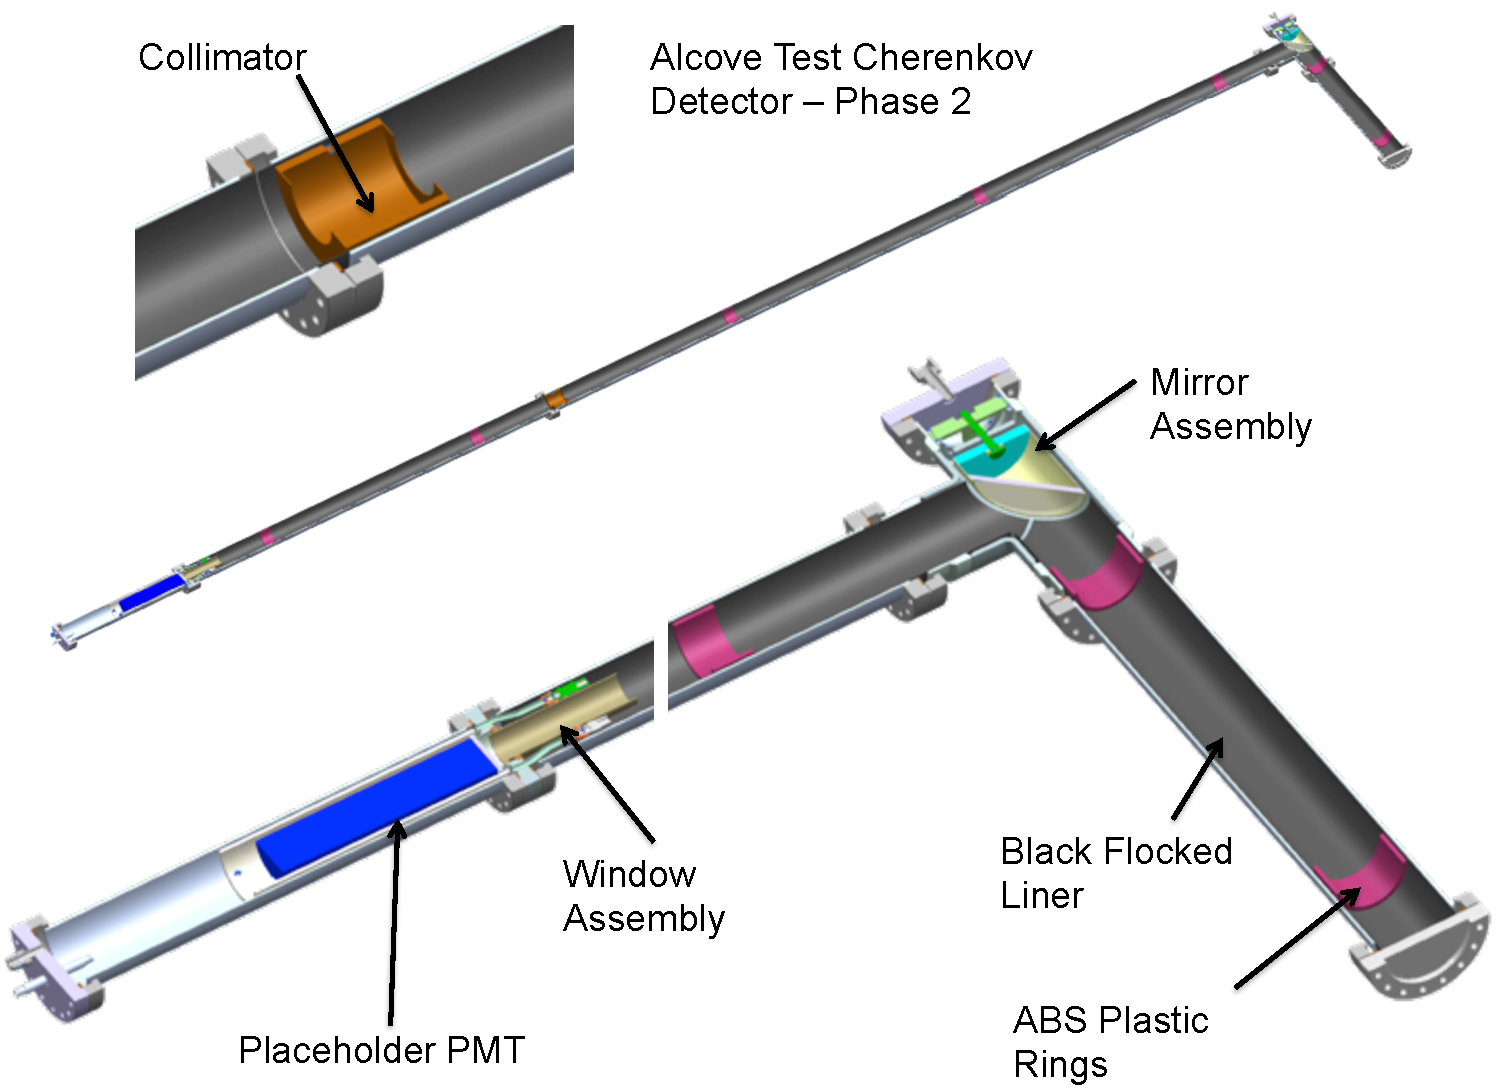
\includegraphics[width=4in,angle=0]{CherenkovCounterDetail}
\end{cdrfigure}

A full description of the BLM prototyping plan may be found in Section~\ref{sec:proto-nd-blm}.
A prototype Cherenkov counter, along with associated fully automated gas systems,
HV systems, and data acquisition system has been constructed and is undergoing
testing in the NuMI neutrino beam's muon alcove 2. In addition, three diamond
detectors~\cite{ref:CERNdiamond} for ionization measurements have also been installed into the alcove.
%Figure~\ref{fig:Alcove2Cherenkov} shows the prototype detectors in NuMI alcove 2.
A second set of muon detectors, the final DUNE design, are being constructed at this time (2015). They are being installed directly behind the NuMI proton beam dump (muon alcove 1). They will be mounted on a movable stand, and the entire setup will be eventually transferred the DUNE absorber hall. The higher radiation environment of alcove 1 will be more similar to the eventual DUNE installation. It will allow the DUNE muon detectors to be calibrated in the NuMI beam and ready for use in the DUNE beam.

%\begin{cdrfigure}[Muon gas Cherenkov counter]{Alcove2Cherenkov}{A prototype muon gas Cherenkov detector for DUNE.  Muons travel through an L-shaped 4" Conflat pipe filled with a pressurized gas. A flat mirror mirrors directs the optical photons to a photo multiplier. The lower right inset shows the 20 bar MKS pressure reading achieved by the Cherenkov gas system, and the inset on the upper right shows the CERN/Cividec diamond detectors mounted to the Cherenkov housing.}
%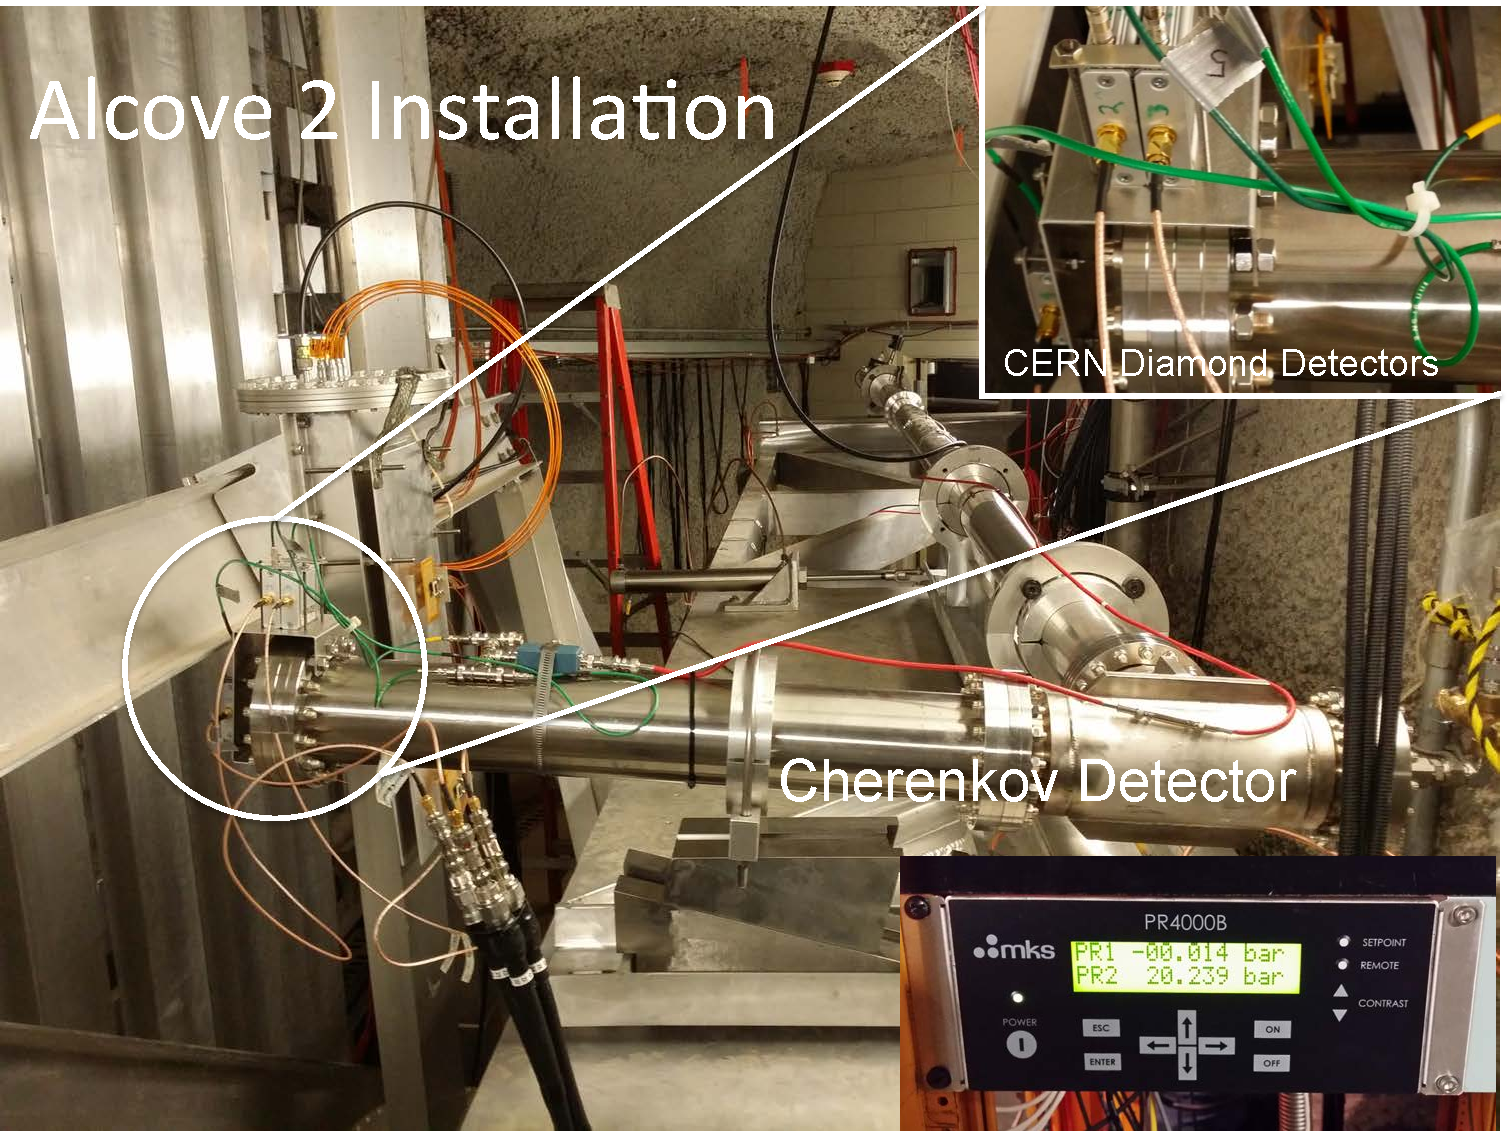
\includegraphics[width=4in]{Alcove2Cherenkov}
%\end{cdrfigure}

% This material was moved to the proto-nd.tex file under the section on prototyping
%
%A prototype Cherenkov counter, along with associated fully automated gas systems,
%HV systems, and data acquisition system has been constructed and is undergoing
%testing in the NuMI neutrino beam's muon alcove 2. In addition, three diamond
%detectors~\cite{ref:CERNdiamond} for ionization measurements have also been installed into the alcove.
%Figure~\ref{fig:Alcove2Cherenkov} shows the prototype detectors in NuMI alcove 2.
%
%The counter is constructed with a 1 meter long radiator section
%as shown in Figure~\ref{fig:CherenkovCounterDetail} . A 20 foot extension allows the reflected 
%Cherenkov light to travel to a sapphire pressure window viewed by a photo multiplier tube.
%
%The prototype is now fully integrated into NuMI operations and real-time waveforms can be viewed online as shown in Figure~\ref{fig:MuonDetectorWaveforms}. The top panel shows the waveform from the Cherenkov counter at 2 atm gas pressure, that corresponds to a muon momentum threshold of 3 GeV/c. The second panel shows the waveform from a $9mm\ \times\ 9mm$ diamond detector mounted to the front flange of the Cherenkov radiator section as shown in the inset 
%of Figure~\ref{fig:Alcove2Cherenkov}.
%
%\begin{cdrfigure}[Muon gas Cherenkov counter]{Alcove2Cherenkov}{A prototype muon gas Cherenkov detector for DUNE.  
%Muons travel through an L-shaped 4" Conflat pipe filled with a pressurized gas. A flat mirror mirrors directs the optical photons to a photo multiplier. The lower right inset shows the 20 bar MKS pressure reading achieved by the Cherenkov gas system, and the inset on the upper right shows the CERN/Cividec diamond detectors mounted to the Cherenkov housing.}
%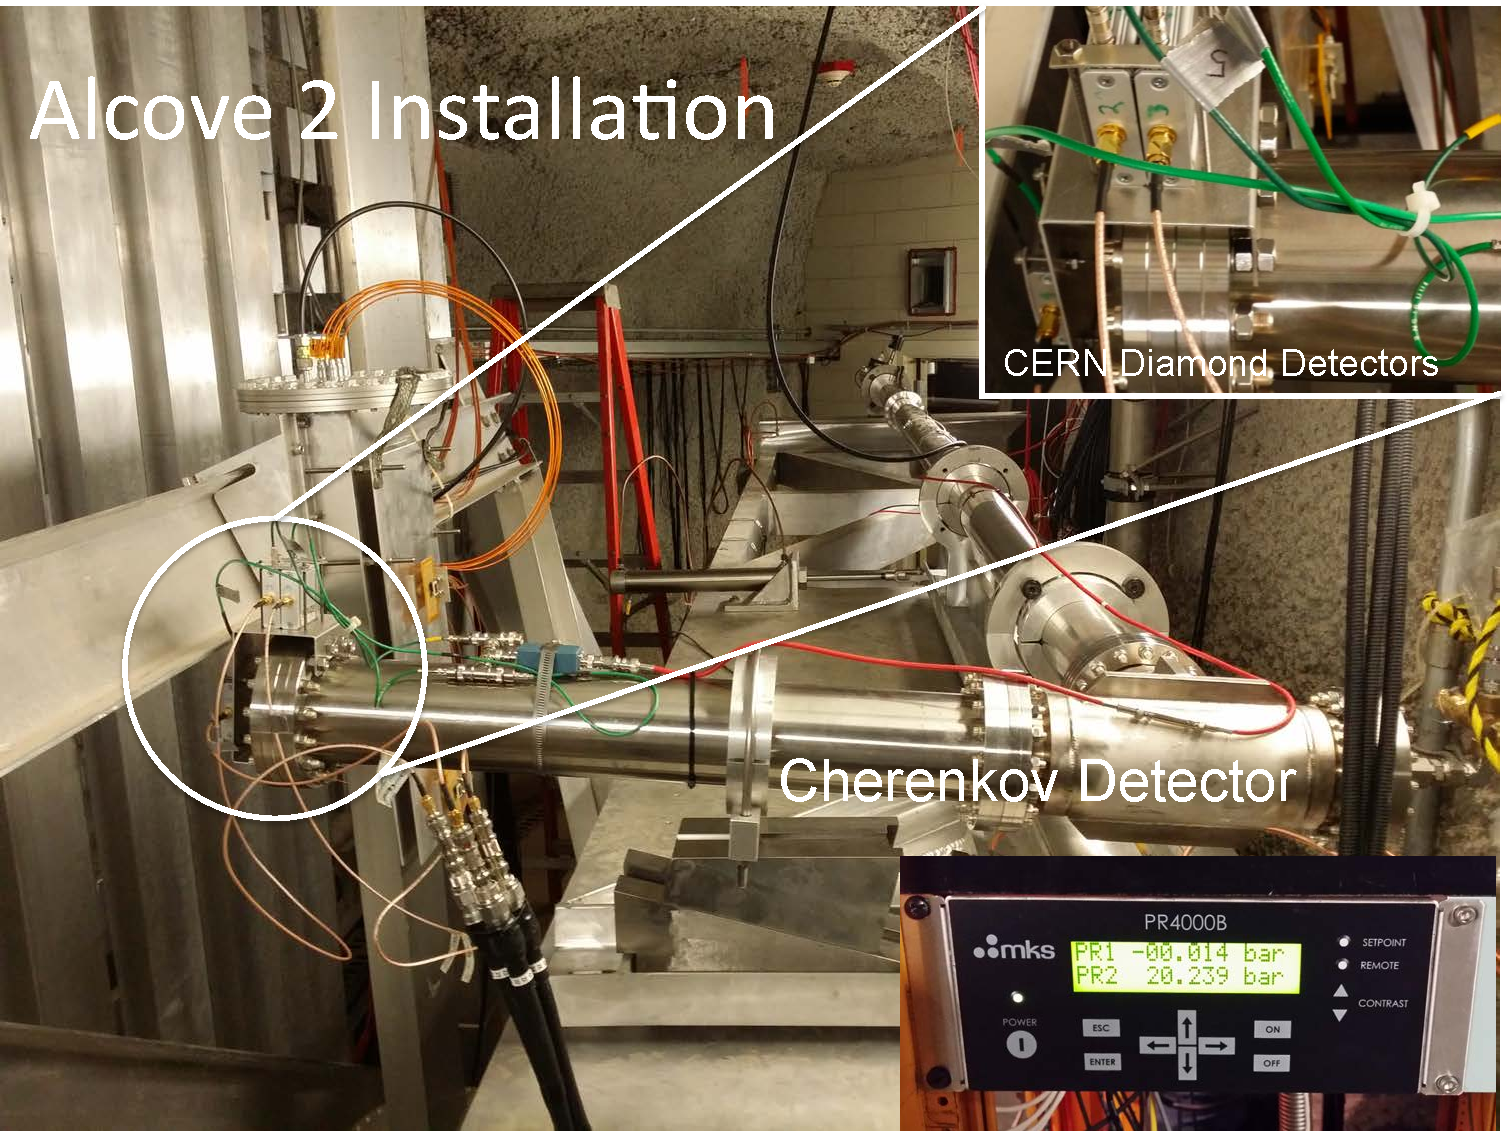
\includegraphics[width=4in]{Alcove2Cherenkov}
%\end{cdrfigure}
%
%\begin{cdrfigure}[Muon Detector Waveforms]{MuonDetectorWaveforms}{The realtime display of the
%muon detector prototypes in operation on the NuMI beam line. The top two panels are the Cherenkov counter and CERN diamond detector \cite{ref:CERNdiamond}, The signals are transmitted through low-loss heliax cable, and then the waveform is digitized at 2.5 GHz with a 12 bit dynamic range, and the recorded onto disk storage for analysis. The signal from the muons is contained in the short beam pulse "buckets" created by the accelerator RF structure. The fast timing allows the prompt muon signal to be easily separated from potential backgrounds such as stopped muon decays, beta decays, and neutrons.}
%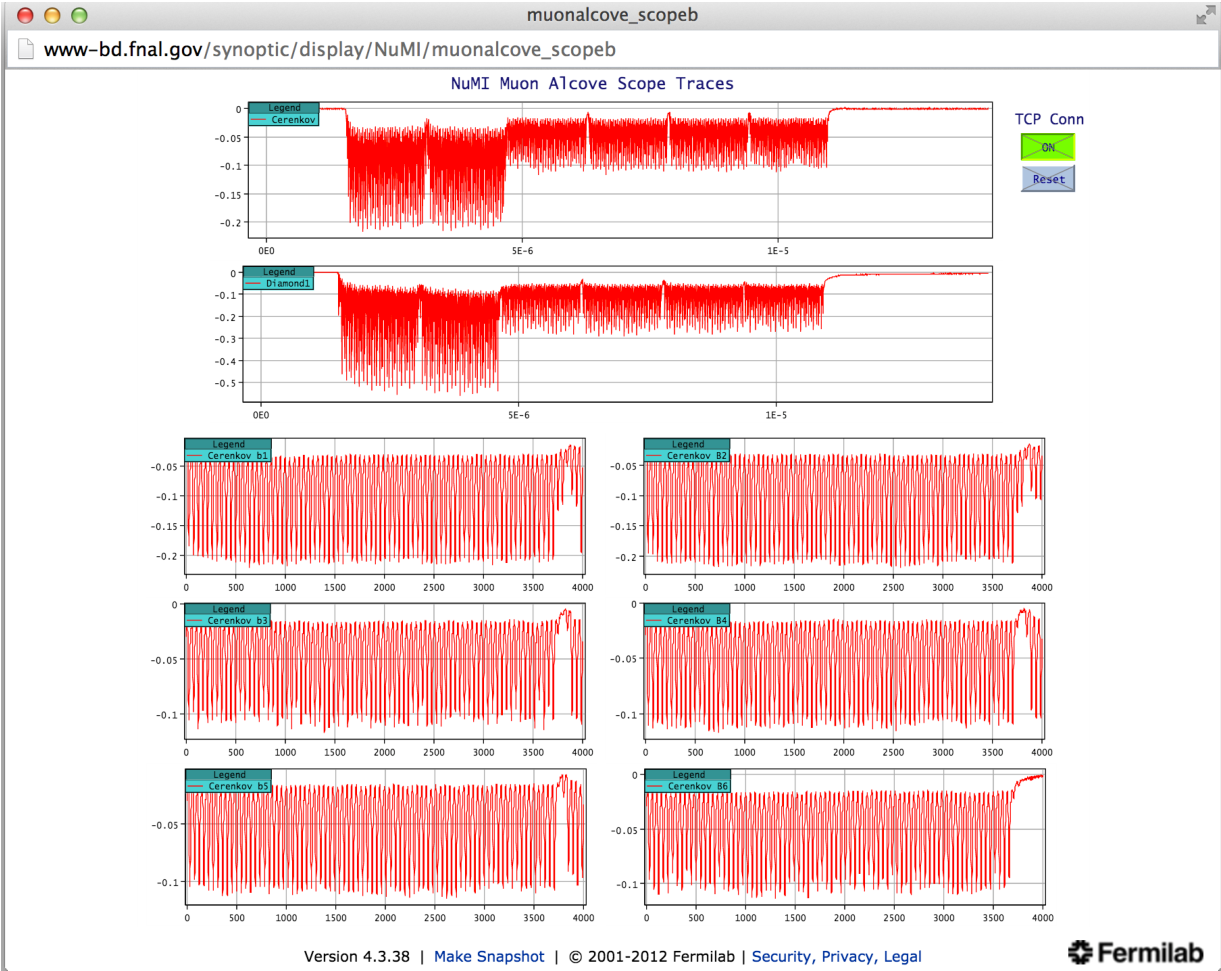
\includegraphics[width=4in]{MuonDetectorWaveforms}
%\end{cdrfigure}
%
%A second set of muon detectors, the final DUNE design, are being constructed at this time (2015). They are being installed directly behind the NuMI proton beam dump (muon alcove 1). They will be mounted on a movable stand, and the entire setup will be eventually transferred the DUNE absorber hall. The higher radiation environment of alcove 1 will be more similar to the eventual DUNE installation. It will allow the DUNE muon detectors to be calibrated in the NuMI beam and ready for use in the DUNE beam.
%\subsection{Installation}
%
%Installation will begin following the absorber installation and the installation of the stopped muon systems
%systems. The counters will be removed from the NuMI Alcove 1 area after calibration in the NuMI beam, and then 
%stored until they are needed for DUNE. 
%The gas handling system will be located nearby, also on the lower level of the Absorber Hall.


%
%
%%%%%%%%%%%%%%%%%%%%%%%%%%%%%%%%%%%%%%%%%%%%%%%%%%%%%%%
\subsection{Muon Ionization Detector Reference Design}
\label{sec:detectors-nd-blm-muon-ionization}

DUNE is in the process of evaluating CVD diamond detectors
as ionization measurement devices. Their advantage is two-fold, they are much more
radiation resistant than silicon, and they provide a much faster signal than ion chambers
which allows them to distinguish between background and the prompt muon signal. 
The DUNE NDC plans to use the ionization devices, e.g. CVD diamond, to monitor
the beam stability, direction and shape, 
and also potentially to determine the absolute flux of muons or to determine the 
muon-energy spectrum. Instead, the stopped-muon counters %(WBS 130.03.03.02) 
and gas Cherenkov detector %(WBS 130.03.03.04) 
will be used, respectively, to determine the flux and energy
spectrum of the muons. 

The reference conceptual design is to use CVD diamond ionization detectors arranged in two
arrays. Each array will measure the centroid of the muon beam to insure a stable neutrino flux
at the near and far detectors. The detectors are arranged in a diamond shaped arrays as shown in 
Figure~\ref{fig:AbsorberPerspectiveOverview2} and Figure~\ref{fig:CherenkovStandView}.

\begin{cdrfigure}[Model of ionization detector layout]{CherenkovStandView}{A model of the ionization detector layout behind the Cherenkov detector stand showing the 13 detectors in a grid configuration.}
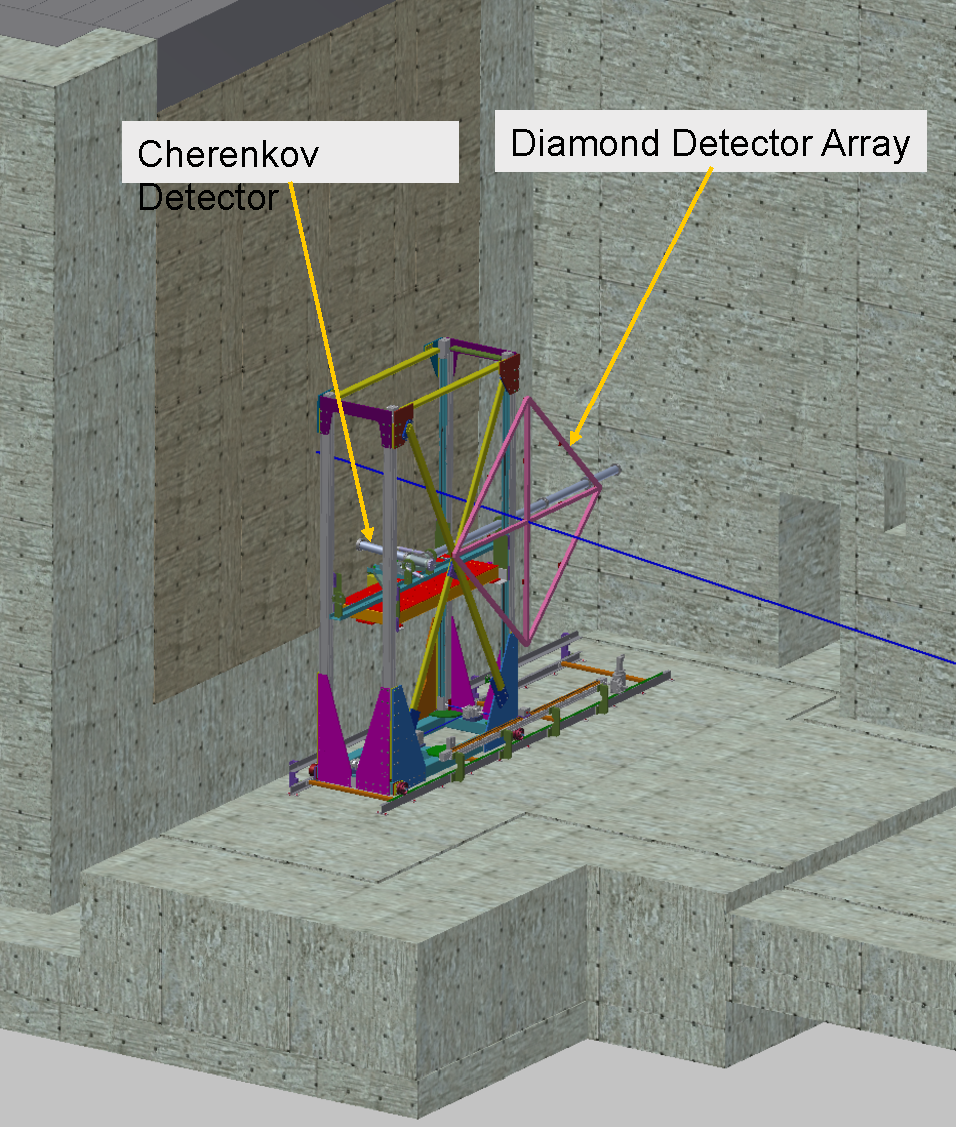
\includegraphics[width=2.5in,angle=0]{CherenkovStandView}

\end{cdrfigure}

The reference design for DUNE includes two arrays of ionization counters, one 
behind the absorber and a second one behind steel shielding blocks. 
DUNE wants to achieve a precision in the beam center of 0.2~milliradians
(5~cm for a 250~m decay pipe). A quick study has 
determined the sensitivity for various arrangements of the ionization counters for each layer and
shows the typical precision such a system can achieve is of order 1cm.

It will be necessary to be able to monitor this ratio in DUNE on a spill-by-spill 
basis to look for signs of target degradation or horn failure.  
Therefore, a second ionization array, placed behind several layers of 
shielding blocks, will be necessary.  In Figure~\ref{fig:AbsorberPerspectiveOverview2}
the second array is placed behind 4 m of steel shielding.  
Since the density of steel is roughly 3 times larger than that of rock, 
this is comparable to the depth of the NuMI second muon alcove, which sits behind 12 m of rock.  
More detailed studies will need to be performed to determine 
if this is the optimal location for sensitivity to changes in the target density.

The prototype testing of the diamond detectors is described in the 
Section~\ref{sec:proto-nd-blm}. For the DUNE ionization detectors, a small array of prototype
counters will be built and operated in the existing NuMI
alcove 1 to determine the optimal design and operating conditions for
the DUNE monitors. This will be done in 2016 and 2017. 
It will provide a good field test in roughly the same environment as expected during DUNE
operations. It will also be cross-checked against the existing NuMI
muon-monitoring system.  The goals of these tests are to understand the linearity 
of the response of these counters (by comparing the observed signal to variations in the beam intensity), their long-term stability and operational reliability.  


%
%
%%%%%%%%%%%%%%%%%%%%%%%%%%%%%%%%%%%%%%%%%%%%%%%%%%%%%%%
\subsection{Stopped Muon Detector Reference Design} % (WBS 130.03.03.02)}
\label{subsec:detectors-nd-blm-stopped-mu}

The second system under development is stopped-muon counters, also called
Michel-electron detectors. This method will measure the muon flux without
suffering from some of the disadvantages intrinsic to systems that
detect through-going muons. The strategy employed here is to stop muons
in a material with significant carbon content 
and, via muon capture, to produce $^{12}B$ that will in turn undergo $\beta$ decay.
 The high-carbon material, in this case graphite, surrounds a Cherenkov radiator
material which is sensitive to electrons from muon decay or 
high-energy beta decays.  Figure~\ref{fig:StoppedMuonCounterDetail} 
shows the conceptual design of a single stopped-muon counter. 


\begin{cdrfigure}[Michel-electron detector conceptualization]{StoppedMuonCounterDetail}{Conceptual design of a single Michel-electron detector (stopped-muon counter)}
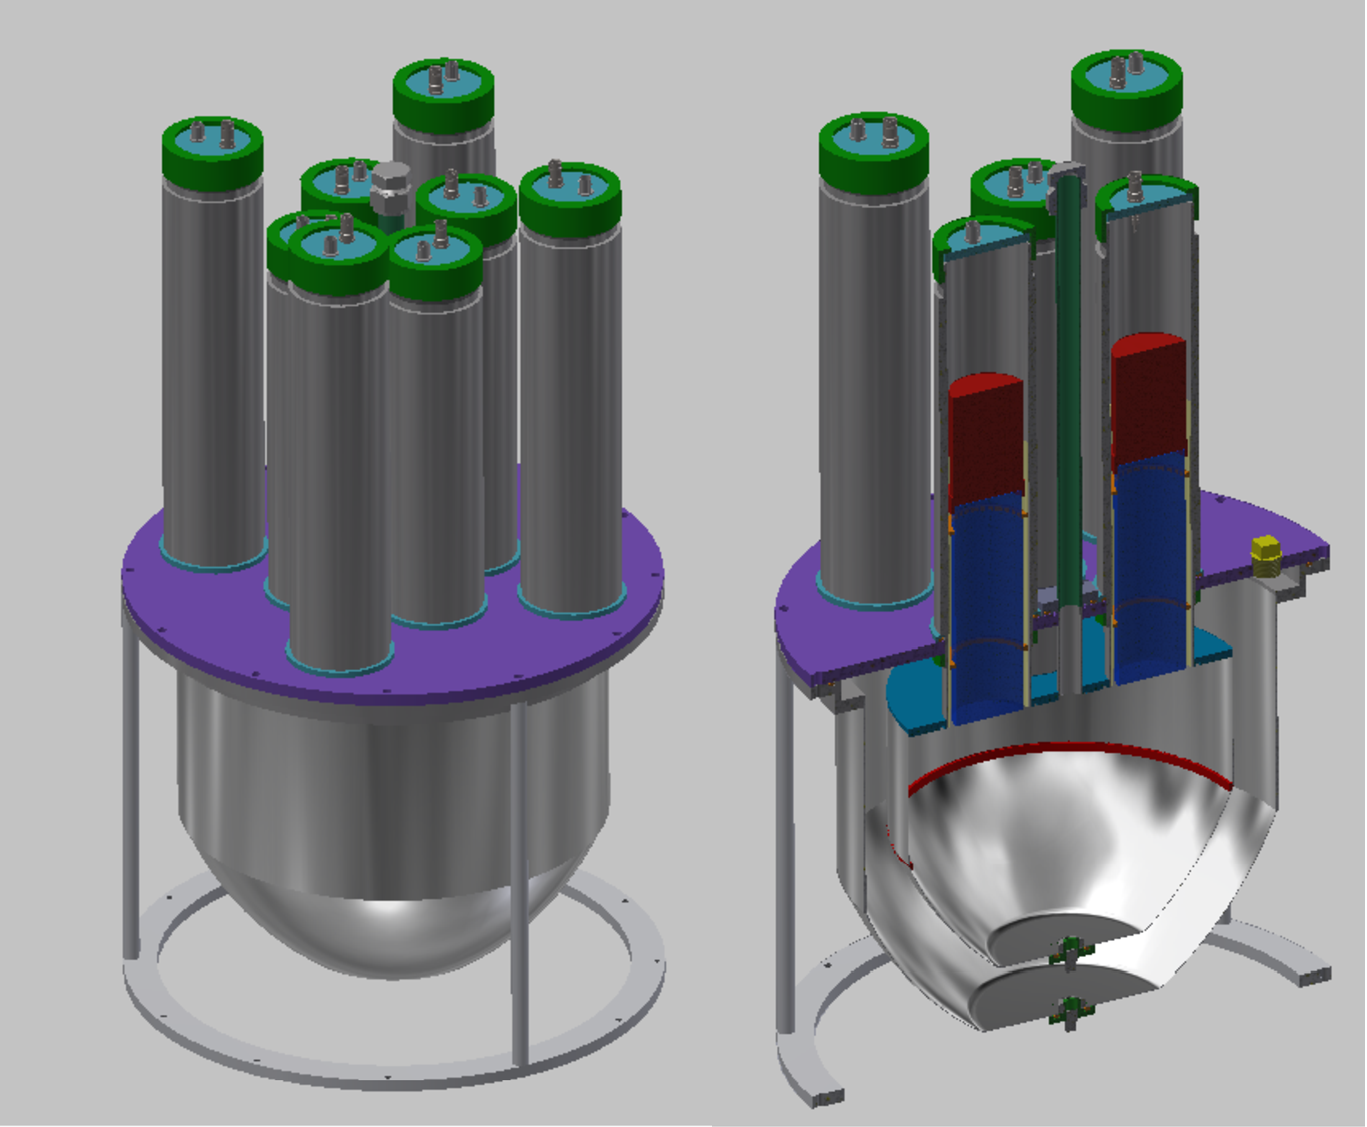
\includegraphics[width=3in,angle=0]{StoppedMuonCounterDetail}
\end{cdrfigure}

The stopped muon detectors will only operate in the lower-rate
environment that is present several muon lifetimes (2.2 $\mu s$) after the beam pulse is
over. There are two possible modes for this type of system. 
The first is an integrating mode where the characteristic decay time of 
2.2~$\mu s$ for muon decay and corresponding beta-decay lifetimes is used to
unfold the total number of decays. The other mode under
investigation uses the ability to record individual decays rather
than an analog current measurement. This mode may allow a more precise absolute
normalization of the flux and fit the muon lifetime in the Michel-electron detector. 
This will provide a more robust cross-check on the
muon signal than will ionization detectors, which are sensitive to delta
rays, photon conversions and other charged particles.

Besides the Michel decays of stopped muons, the system will
independently measure both the $\mu ^{+}$ and $\mu ^{-}$ stopped
rates as a function of depth. 
While the 2.2~$\mu $s decay time of the $\mu^+$ is a reliable
signature, in mineral oil roughly 8.5\% of the $\mu^{-}$ undergo capture
on the $^{12}C$ nucleus, and 15\% of those leave behind a $^{12}B$
ground state nucleus. That $^{12}B$ nucleus will undergo $\beta$ decay
with a half-life of 20.20~ms and an electron spectrum with an endpoint
of 13~MeV. This signal is expected to yield a reliable measurement of the rate of stopped
$\mu^{-}$.

The stopped-muon detector reference design
is modular and based on a Cherenkov radiator of
minimum size to contain a 52.8-MeV electron and distinguish it cleanly
from lower-energy radioactivity. This conceptual design employs
a liquid mineral oil  radiator. The radiator will be coupled to four photomultiplier tubes (PMT) or
other photon counter.  The entire module will be surrounded by a 
liquid scintillator veto layer, and the entire module then
encased in a material that provides both a uniform-density stopping
target for muons and some shielding from incoming neutrons. One or two
signal channels will be associated with each module, and the full
waveform from each channel over approximately 100~ms will be recorded
on each beam pulse.

Nine modules will be placed just behind the absorber in a cross pattern.  An additional 12 will be 
placed at multiple depths in the shielding in order to sample the muon flux
from different energies, as shown in Figures~\ref{fig:AbsorberElevationView}. 
The shielding will simultaneously act to range out the muons and shield the detectors from 
neutrons. The Cherenkov light from Michel-decay electrons will exit the 
counter and be collected by either nearby PMTs or by a light guide which will
guide the light to a remote optical sensor.  

 A full description of the prototyping plan can be found in Section~\ref{sec:proto-nd-blm}.
The prototypes will be installed into the alcoves in 2016 and 2017.
Studies will be performed to determine if the photon sensors
can survive the radiation environment at the location of the Michel
detector. If the sensors can survive, they can be attached directly to
the Cherenkov medium; if not, optical guides will have to bring the
light to a lower-radiation area to the side of the beam. Potential
radiation damage to the Cherenkov radiator itself will also be
studied.

\subsection{Installation and Operation}

The muon system detectors, already fully calibrated in the NuMI beam,
will be installed as soon as the absorber hall (LBNF-30) is ready.
Because the system will be located in a radiation-controlled
environment that will not be accessible during beam operation, it is
essential that the electronics and gas handling system be both robust
and remotely operable.  The prototype system in use at the NuMI area can be relocated for that purpose,
or if desired a new system may be constructed.
Periodic access will be required to the utilities area to replace gas bottles.

The blue blocks associated with the muon systems will be installed first.
The positioned stand for the Cherenkov detector system will be installed next.
and then the various detectors will be installed.
The stopped-muon counters will be placed into the spaces between the blue-block walls on
support frames.   There will be access to the areas between the shield blocks 
from the side, and the stopped-muon counters will be designed so that they can 
be wheeled in from the side.  If needed, they could then be moved around to measure
the stopped-muon rates across the muon beam.

The muon systems will be operated continuously in order to insure a stable,
high quality neutrino beam.
The muon-monitor-system data will be displayed in the control room on
a spill-by-spill basis to monitor the beam stability. Because the
system will be located in a radiation-controlled environment that will
not be accessible during the beam operation, it is essential that the
electronics be designed for remote operation.

\section{Hadron Production Measurements}
\label{sec:detectors-nd-ref-hadron}

\subsection{Introduction}

The technical components that would be needed to implement the strategies 
described in this chapter are outside the scope of the DUNE NDS conceptual 
design. This information is included in this document because it complements the conceptual 
design and expands the NDS capabilities to more closely meet the mission need without increasing the project cost.

\subsection{External Hadron-Production Measurements}
\label{sec:detectors-nd-external-hadron}

Uncertainties on hadron production will translate into uncertainties in the neutrino fluxes
in the DUNE Far Detector, since the neutrinos are produced by hadrons decaying in the decay pipe. Precise calculations of neutrino fluxes in high-energy accelerator beams are limited
at present by our knowledge of hadron production cross-sections in hadron-nucleus collisions. 
The modeling of strong-interaction cascades and hadronic yields from ``thick'' targets
(up to a couple of interaction lengths) relies on detailed knowledge of underlying physics
and cross-sections, which must be provided as a starting point to simulations. The resulting 
prediction of the flux of neutrinos, produced from decays of pions, kaons, and muons
emerging from a hadronic shower and beam line re-interactions, is an essential part
of simulations of most neutrino experiments. 

Two-detector neutrino oscillation experiments 
predict the neutrino flux at the far detector by using neutrino fluxes ``calibrated'' (or
appropriately scaled) by event energy spectra measured in the near detector. However, even
these experiments must rely on the beam simulations since the decay pipe (where most beam
neutrinos are created) provides different angular acceptance for the two detectors. In addition, 
experiments using near and far detectors based on different detection technologies further complicate the extrapolation. This chapter outlines the DUNE strategy for augmenting the capabilities of the BLM with
external measurements of secondary-beam particles. 
%\fixme{This was originally written when we just had 
%the BLM and no NND; no change needed here? Second point: This sentence should be in the intro paragraph of this chapter.}

\subsection{Background}

A complete knowledge of the momenta and decay points of the kaons, pions and
muons would be sufficient to completely predict the un-oscillated flux of neutrinos
at the Near and Far Detector locations. This would require knowledge of:

\begin{itemize}
\item the phase-space distribution of the initial proton beam
\item details of all materials present in the target, horn and decay pipe areas
\item  the electromagnetic focusing characteristics of the magnetic horn
\item the detailed development of the hadron cascade, spawned by the
initial proton, that passes through the target/horn/decay pipe
\item the meson-to-neutrino decay rates
\end{itemize}

With careful engineering design and careful control of the materials in the target
area, all of these items can be simulated accurately except hadronic cascades in
the target, horn and decay pipe. The simulation of the hadronic cascade requires
accurate knowledge of the hadron scattering cross sections, for which there are no
first-principle calculations. These cross sections must therefore rely on models, which
in turn require hadron-production measurements that span particle type, particle
energy and the various materials found in the target, horn and decay pipe.

At the present time, a sufficient body of hadron-production measurements does
not exist to achieve DUNE's desired accuracy of 4-5\%, as determined by the irreducible error on the statistical uncertainty for the appearance-measurement back-ground, although this is expected to improve over time. As the BLM system described in Chapter~\ref{ch:nd-blm} cannot meet this requirement alone, a near-far comparison
will be more complicated than in certain other neutrino-oscillation experiments, e.g.,
MINOS experiment~\cite{gnumi-validation}.


\subsection{The US-NA61/SHINE Program}
\label{sec:detectors-nd-blm-external-usna61}

A proposal to make measurements for the Fermilab neutron program with the NA61/SHINE experiment has been funded by DOE/HEP \cite{ref:NA61Proposal,ref:NA61Addendum} , US-NA61, and recommended by the CERN SPSC. NA61/SHINE is situated in the North Area of CERN on the H2 beam line. 

The detector, schematically shown in Figure~\ref{fig:NA61Scheme} is comprised of two large air gap, Helmholtz-coil superconducting magnets with a total bending power of 9 T-m. The detector is instrumented with gas TPC tracking, time-of-flight counters, and a hadron calorimeter (at very forward angles). The US-NA61 measurements will provide hadron-production data sufficient for predicting neutrino fluxes at DUNE. A pilot run of 120~GeV/c protons interacting on a thin 4\% graphite target was taken by NA61 during July, 2012. A 4-week dedicated physics run is scheduled for October, 2015.

The run plan for the 2015 data is shown in the table in Figure~\ref{fig:NA61RunPlan}. The initial run will focus on proton and pion data at 120 GeV/c and 60 GeV/c energies. This will constrain well extrapolations from higher and lower energies that are currently under use in neutrino beam simulations.

\begin{cdrfigure}[A schematic drawing of the CERN NA61 detector]{NA61Scheme}{A schematic drawing of the CERN NA61 detector, a hadron production and heavy ion experiment designed to measure hadrons over a large part of the relevant phase for neutrino experiments. The TPCs, shown in blue, can separate pions from protons and kaons.}
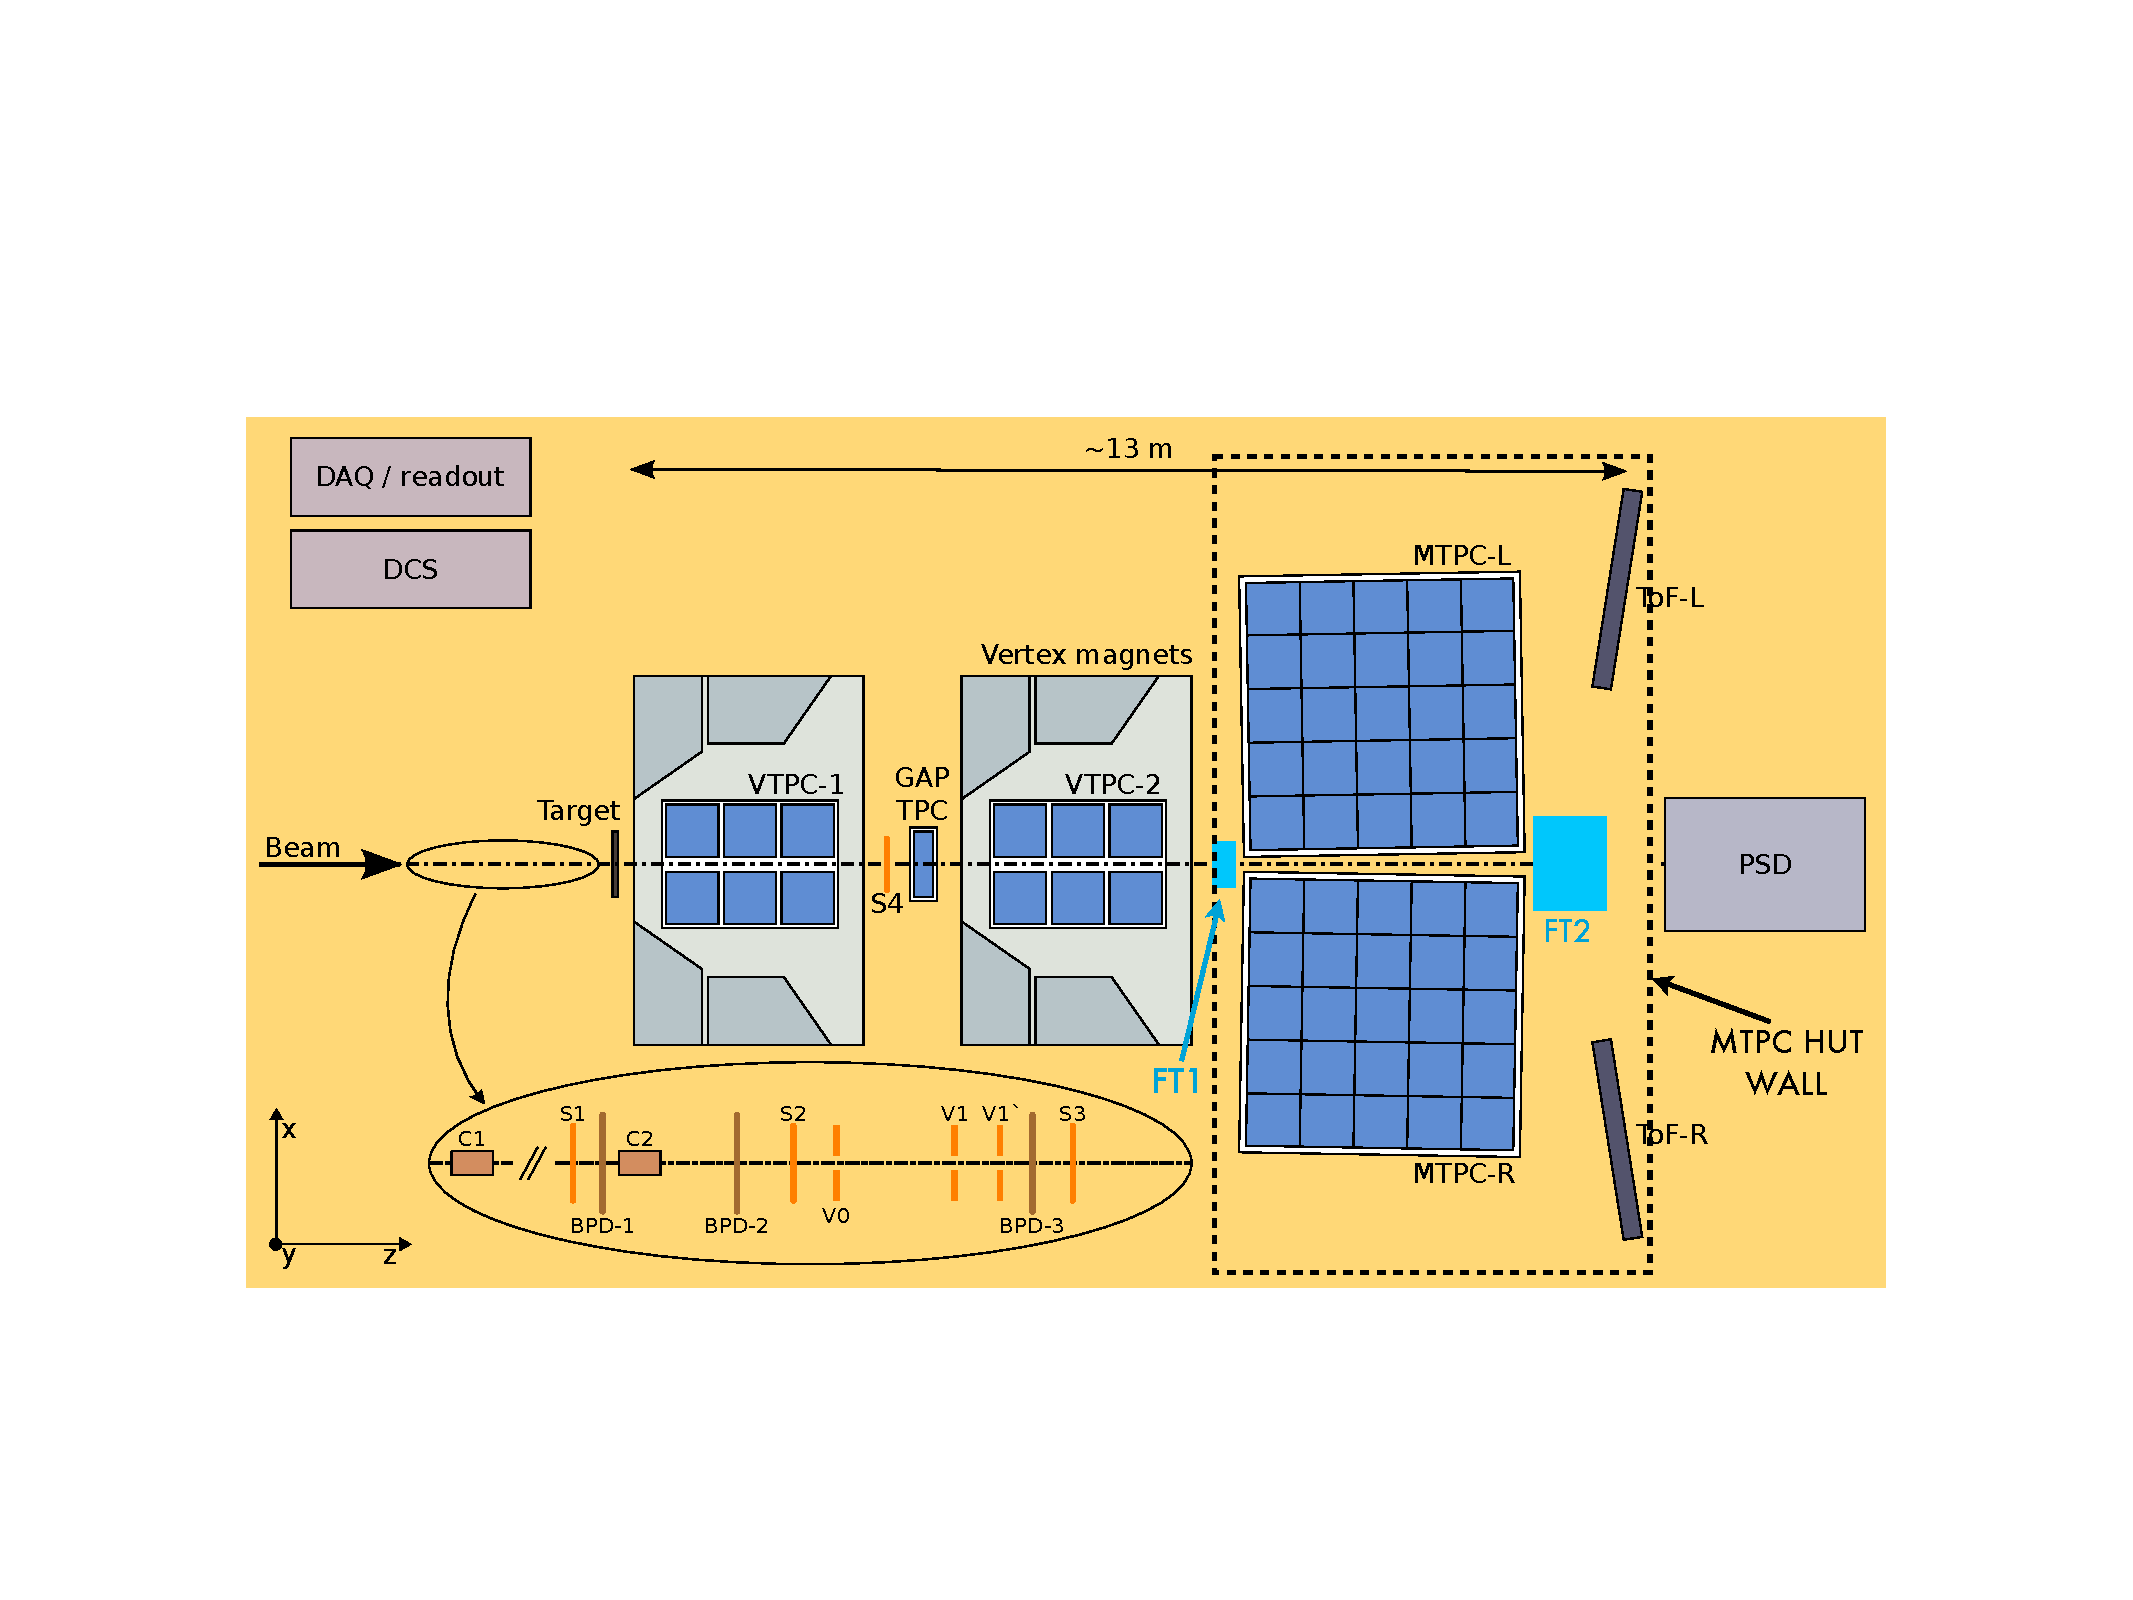
\includegraphics[width=4in]{NA61-PlanView}
\end{cdrfigure}

\begin{cdrfigure}[The 2015 run plan for US-NA61.]{NA61RunPlan}{A table that shows the proposed run plan for 
the US-NA61 data run in the fall of 2015.}
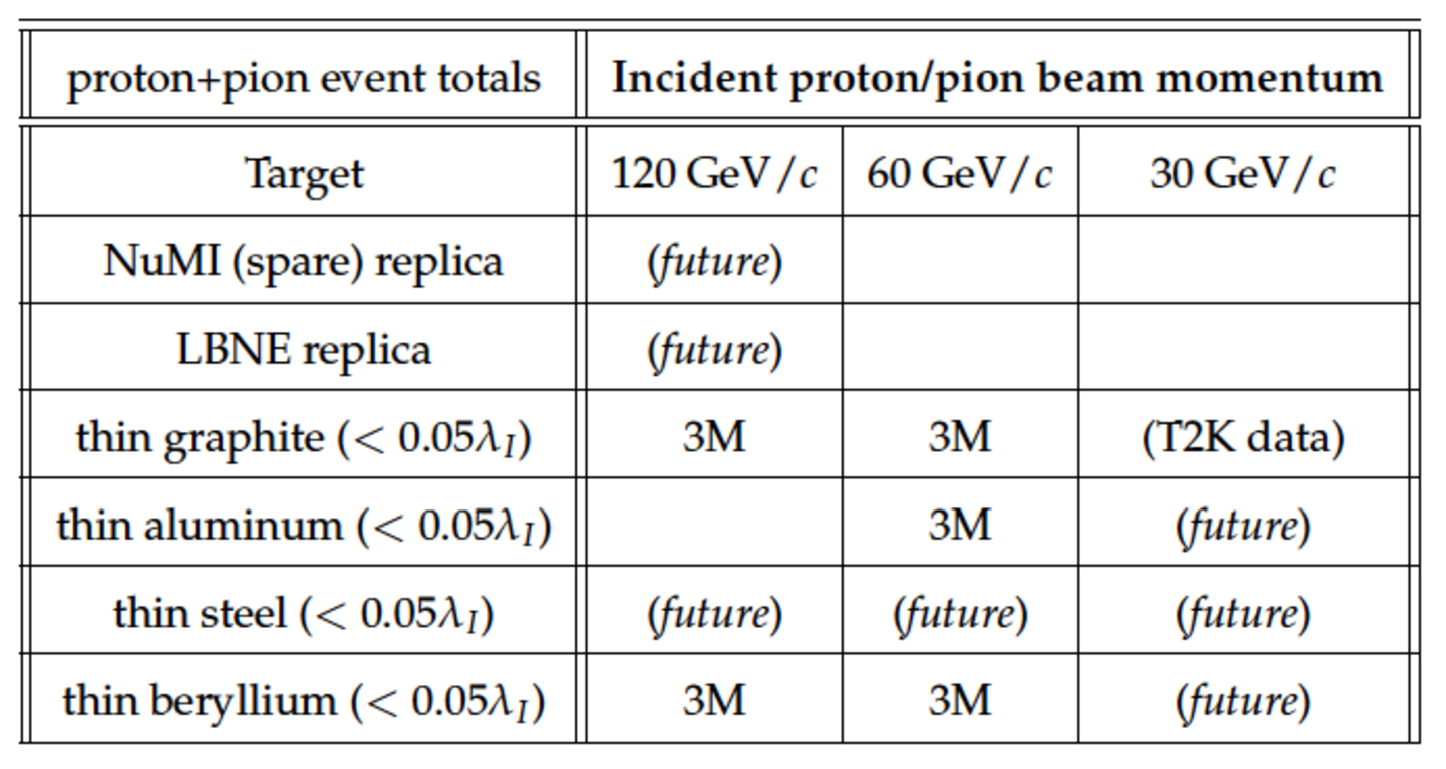
\includegraphics[width=4in]{NA61RunPlan}
\end{cdrfigure}

